\documentclass[GTSResumen.tex]{subfiles}
%\usepackage{amsmath,amssymb}
%\usepackage[utf8]{inputenc}
%\usepackage[spanish]{babel}
%\usepackage[]{graphicx}
%\usepackage{enumerate}
%\usepackage{amsthm}
%\usepackage{tikz-cd}
%\usetikzlibrary{babel}
%\usepackage{pgf,tikz}
%\usepackage{mathrsfs}
%\usetikzlibrary{arrows}
%\usetikzlibrary{cd}
%\usepackage[spanish]{babel}
%\usepackage{fancyhdr}
%\usepackage{titlesec}
%\usepackage{floatrow}
%\usepackage{makeidx}
%\usepackage[tocflat]{tocstyle}
%\usetocstyle{standard}
%%\usepackage[sc]{mathpazo}
%%\usepackage{blindtext}
%\usepackage{color}   %May be necessary if you want to color links
%\usepackage{hyperref}
%\hypersetup{colorlinks=true,citecolor=red, linkcolor=blue}
%
%
%\renewcommand{\baselinestretch}{1,4}
%\setlength{\oddsidemargin}{0.25in}
%\setlength{\evensidemargin}{0.25in}
%\setlength{\textwidth}{6in}
%\setlength{\topmargin}{0.1in}
%\setlength{\headheight}{0.1in}
%\setlength{\headsep}{0.1in}
%\setlength{\textheight}{8in}
%\setlength{\footskip}{0.75in}
%
%\newtheorem{teorema}{Teorema}[section]
%\newtheorem{defi}[teorema]{Definición}
%\newtheorem{coro}[teorema]{Corolario}
%\newtheorem{lemma}[teorema]{Lema}
%\newtheorem{ej}[teorema]{Ejemplo}
%\newtheorem{ejs}[teorema]{Ejemplos}
%\newtheorem{observacion}[teorema]{Observación}
%\newtheorem{observaciones}[teorema]{Observaciones}
%\newtheorem{prop}[teorema]{Proposición}
%\newtheorem{propi}[teorema]{Propiedades}
%\newtheorem{nota}[teorema]{Nota}
%\newtheorem{notas}[teorema]{Notas}
%\newtheorem*{dem}{Demostración}
%\newtheorem{ejer}[teorema]{Ejercicio}
%\newtheorem{consec}[teorema]{Consecuencia}
%\newtheorem{consecs}[teorema]{Consecuencias}
%
%\providecommand{\abs}[1]{\lvert#1\rvert}
%\providecommand{\norm}[1]{\lVert#1\rVert}
%\providecommand{\ninf}[1]{\norm{#1}_\infty}
%\providecommand{\numn}[1]{\norm{#1}_1}
%\providecommand{\gabs}[1]{\left|{#1}\right|}
%\newcommand{\bor}[1]{\mathcal{B}(#1)}
%\newcommand{\R}{\mathbb{R}}
%\newcommand{\N}{\mathbb{N}}
%\newcommand{\Q}{\mathbb{Q}}
%\newcommand{\C}{\mathbb{C}}
%\newcommand{\Pro}{\mathbb{P}}
%\newcommand{\Tau}{\mathcal{T}}
%\newcommand{\verteq}{\rotatebox{90}{$\,=$}}
%\newcommand{\vertequiv}{\rotatebox{110}{$\,\equiv$}}
%\providecommand{\lrg}{\longrightarrow}
%\providecommand{\func}[2]{\colon{#1}\longrightarrow{#2}}
%\newcommand*{\QED}{\hfill\ensuremath{\blacksquare}}
%\newcommand*\circled[1]{\tikz[baseline=(char.base)]{
%            \node[shape=circle,draw,inner sep=1.5pt] (char) {#1};}}
%\newcommand*{\longhookarrow}{\ensuremath{\lhook\joinrel\relbar\joinrel\rightarrow}}
% \newenvironment{solucion}{\begin{trivlist}
%\item[\hskip \labelsep {\textit{Solución}.}\hskip \labelsep]}{\end{trivlist}}
%
%\def\quot#1#2{%
%    \raise1ex\hbox{$#1$}\Big/\lower1ex\hbox{$#2$}%
%}
%
%\makeatletter
%\renewcommand\tableofcontents{%
%  \null\hfill\textbf{\Large\contentsname}\hfill\null\par
%  \@mkboth{\MakeUppercase\contentsname}{\MakeUppercase\contentsname}%
%  \@starttoc{toc}%
%}
\setcounter{chapter}{2}
%\pagestyle{fancy}
%\fancyhf{}
%\rhead{Geometría y Topología de Superficies (Grado en Matemáticas)}
%\lhead{Curso 2016/2017}
%\cfoot{\thepage}
%
\begin{document}
%%\title{Geometría y Topología de Superficies}
%%\author{Antonio Quintero Toscano\\ Javier Aguilar Martín}
%%\date{Curso 2016/2017}
%%\maketitle
%
\renewcommand\chaptername{\Huge Tema}
%
\titleformat{\chapter}[display]
    {\normalfont\huge\bfseries}{\chaptertitlename\ \thechapter}{10pt}{\Huge}
\titlespacing*{\chapter}{0pt}{-1cm}{10pt}
%
%\tableofcontents
\chapter{Teoría de Homotopía}

\section{Homotopía}
Vamos a introducir el concepto de deformación de curvas cerradas (``lazos"). La idea es fijar un punto y variar el lazo de manera continua sin mover el punto. Comenzamos formalizando la idea de deformar una función en otra con el tiempo. 

\begin{defi} Sean $f,g\func{X}{Y}$ funciones continuas y sea $I=[0,1]$. Decimos que $f$ y $g$ son \textbf{homotópicas} ($f\simeq g$) si $\exists H\func{X\times I}{Y}$ continua tal que $H(x,0)=f(x)$ y $H(x,1)=g(x)$. A la aplicación $H$ la llamamos \textbf{homotopía} entre $f$ y $g$. Si una de las funciones es constante, decimos que la otra es \textbf{nul-homotópica}. Si $A\subseteq X$, decimos que $f$ y $g$ son \textbf{homotópicas relativamente} a $A$ si la homotopía $H$ cumple además $H(a,t)=f(a)=g(a)\ \forall a\in A$. Si $A$ es un conjunto unitario hablamos de homotopía \textbf{basada}. En contraposición a la homotopía relativa, a la homotopía que no cumple esa condición se le llama homotopía \textbf{libre}.
\end{defi}

\begin{nota} Si tomamos $A=\emptyset$, la homotopía relativa a $A$ coincide con la homotopía libre.
\end{nota}


\begin{lemma} Ser homotópicas es una relación de equivalencia (también serlo relativamente).
\end{lemma}
\begin{comment}
\begin{dem}\
\begin{itemize}
\item Reflexiva: $f\simeq f$ por $H(x,t)=f(x)$.
\item Simétrica: si $f\simeq g$ por $H\Rightarrow g\simeq f$ por $\widetilde{H}(x,t)=H(x,1-t)$. Se cumplen
\begin{gather*}
\widetilde{H}(x,0)=H(x,1)=g(x)\\
\widetilde{H}(x,1)=H(x,0)=f(x)
\end{gather*}
Se deja como ejercicio probar que $\widetilde{H}$ es continua.
\item Transitiva: sea $f\simeq g$ por $F$ y $g\simeq h$ por $G$. Entonces, $f\simeq h$ por
\begin{equation*}
H(x,t)=\left\{\begin{array}{ccc}
F(x,2t) & si & 0\leq t\leq\frac{1}{2}\\
G(x,2t-1) & si & \frac{1}{2}\leq t\leq 1
\end{array}\right.\Longrightarrow\left\{\begin{array}{c}
H(x,0)=F(x,0)=f(x)\\
H(x,1)=G(x,1)=h(x)
\end{array}\right.
\end{equation*}
Está bien definida en $t=\frac{1}{2}$ pues $F(x,1)=g(x)=G(x,0)$. Se deja como ejercicio probar la continuidad de $H$ y adaptar la demostración al caso relativo.$\QED$
\end{itemize}
\end{dem}
\end{comment}
\begin{lemma}\label{lema} La relación de homotopía es compatible con la composición, es decir, se tienen las siguientes propiedades (que también valen para la homotopía relativa):
\begin{enumerate}
\item[a)] Sean $f,g\func{X}{Y}$, $h\func{Y}{Z}$ continuas. Si $f\simeq g$ entonces $h\circ f\simeq h\circ g$.
\item[b)] Si $h\func{Z}{X}$ y $f,g\func{X}{Y}$ continuas con $f\simeq g$, entonces $f\circ h\simeq g\circ h$.
\item[c)] Si $h,h'\func{Z}{X}$ y $f,g\func{X}{Y}$ con $f\simeq g$ y $h\simeq h'$, entonces $f\circ h\simeq g\circ h'$.
\end{enumerate}
\end{lemma}
\begin{comment}
\begin{dem}\
\begin{enumerate}
\item[a)] Sea $H$ homotopía entre $f$ y $g$. Sea $\widetilde{H}=h\circ H\func{X\times I}{Z}$. Se tiene
\begin{gather*}
\widetilde{H}(x,0)=h(H(x,0))=h(f(x))=(h\circ f)(x)\\
\widetilde{H}(x,1)=h(H(x,1))=h(g(x))=(h\circ g)(x)
\end{gather*}
\item[b)] Sea $\widehat{H}\func{Z\times I}{Y}$ definida como $H\circ(h\times Id)$. Entonces
\begin{gather*}
\widehat{H}(x,0)=H(h(x),0)=f(h(x))=(f\circ h)(x)\\
\widehat{H}(x,1)=H(h(x),0)=g(h(x))=(g\circ h)(x)
\end{gather*}
\item[c)] $f\circ h\underset{a)}{\simeq}f\circ h'\underset{b)}{\simeq}g\circ h'$. Por transitividad de la relación de homotopía $f\circ h\simeq g\circ h'$
\end{enumerate}
$\QED$
\end{dem}
\end{coment}
\begin{defi} Una aplicación $f\func{X}{Y}$ se dice \textbf{equivalencia de homotopía} si $\exists g\func{Y}{X}$ continua tal que $f\circ g\simeq Id_Y$ y $g\circ f\simeq Id_X$. $X$ e $Y$ se dicen entonces \textbf{homotópicamente equivalentes}. En tal caso se dice que $f$ y $g$ son \textbf{inversas homotópicas}.
\end{defi}

\begin{nota} Si $f$ es homeomorfismo, es equivalencia de homotopía, con su inversa como función $g$.
\end{nota}

\begin{ej} $\R^n$ y $\{p\}$ son homotópicamente equivalentes.
\begin{solucion}\
Sea $c\func{\R^n}{\{p\}}$ la función constante $c(x)=p$ y sea $f\func{\{p\}}{\R^n}$ también constante $f(p)=x_0$. Fijamos por comodidad $x_0=0\in\R^n$. Se tiene trivialmente $c\circ f = Id_{\{p\}}\simeq Id_{\{p\}}$. Vamos a probar que $f\circ c\simeq Id_{\R^n}$. Para ello tenemos que definir una homotopía $H\func{\R^n\times I}{\R^n}$. Así pues, definimos la homotopía $H(x,t)=(1-t)x$, con la que se tiene el resultado. \qed
\end{solucion}
\end{ej}

El mismo tipo de aplicación $H(x,t)=(1-t)x$ muestra que todo espacio vectorial normado es homotópicamente equivalente a $\{p\}$. Obsérvese que basta que se trate de un espacio vectorial $V$ dotado de una topología para la cual la aplicación $(v,\lambda)\in V\times\R\longmapsto \lambda v\in V$ sea continua.


\begin{defi} Un espacio $X$ se dice \textbf{contráctil} o \textbf{contractible} si es homotópicamente equivalente a un punto.
\end{defi}
\begin{nota} Todos los espacios vectoriales normados son contráctiles.
\end{nota}

\begin{comment}
\begin{ejer} El cono de cualquier espacio $X$ es contráctil.\

\begin{tikzpicture}[line cap=round,line join=round,>=triangle 45,x=1.0cm,y=1.0cm]
\clip(-3.582960582875703,-0.6860860471104946) rectangle (3,3.385652568344079);
\draw (0.,3.)-- (-1.,0.);
\draw (0.,3.)-- (1.,0.);
\draw [rotate around={0.:(-9.419043382212538E-4,0.)},line width=0.4pt,dash pattern=on 2pt off 2pt] (-9.419043382212538E-4,0.) ellipse (0.9921122128589096cm and 0.35180919174161984cm);
\draw [rotate around={0.:(0.0013947216583214172,0.666816713018603)},line width=0.4pt,dash pattern=on 2pt off 2pt] (0.0013947216583214172,0.666816713018603) ellipse (0.7737037941321484cm and 0.21563538073555172cm);
\draw [rotate around={0.:(0.001394721658320443,1.4)},line width=0.4pt,dash pattern=on 2pt off 2pt] (0.001394721658320443,1.4) ellipse (0.5292944912412179cm and 0.1735358572657806cm);
\draw [rotate around={0.:(-0.003278530334764755,2.2)},line width=0.4pt,dash pattern=on 2pt off 2pt] (-0.003278530334764755,2.2) ellipse (0.2642515780732333cm and 0.1038049712781662cm);
\begin{scriptsize}
\draw [fill=black] (0.,3.) circle (1.5pt);
\draw (0.1,3.2) node[anchor=north west]{$v=[x,1]$};
\end{scriptsize}
\end{tikzpicture}

\end{ejer}
\begin{solucion}
Si $[x,t]\in CX$ es la clase de $(x,t)\in X\times I$, se define $H\func{CX\times I}{CX}$ por $H([x,t],s)=[x,(1-s)t+s]$. Entonces $H([x,t],0)=[x,t]$ y $H([x,t],1)=[x,1]=v$. Queda verificar la continuidad, que se deja como ejercicio. \qed
\end{solucion}
\end{comment}

\begin{ej}
Cualquier convexo $X$ es contráctil, pues basta tomar la homotopía $H(x,t)=(1-t)x+x_0$, con $x_0\in X$ fijo. Esta aplicación está bien definida por ser $X$ convexo.
\end{ej}


\begin{ej} $\R^2\setminus\{0\}$ es homotópicamente equivalente a $S^1$.
\end{ej}
\begin{comment}
\begin{solucion}
Sea $i$ la inclusión $i:S^1\longhookarrow\R^2\setminus\{0\}$ y sea $r\func{\R^2\setminus\{0\}}{S^1}$ dada por $r(x)=\frac{x}{\norm{x}}$. Tenemos que probar que $r\circ i\simeq Id_{S^1}$ y que $i\circ r\simeq Id_{\R^2\setminus\{0\}}$.

\begin{center}
\begin{tikzpicture}[line cap=round,line join=round,>=triangle 45,x=1.0cm,y=1.0cm]
\draw[color=black] (-2,0.) -- (2,0.);
\foreach \x in {-4.,-3.,-2.,-1.,1.,2.,3.,4}
\draw[shift={(\x,0)},color=black] (0pt,-2pt);
\draw[color=black] (0.,-2.5) -- (0.,2);

\clip(-2,-2.5) rectangle (2,2);
\draw [line width=0.4pt] (0.,0.) circle (1.573333333333331cm);
\draw [dash pattern=on 3pt off 3pt] (0.,0.)-- (-0.8924930402912962,-2.0468759302433575);
\draw [dash pattern=on 3pt off 3pt] (0.,0.)-- (1.2136272915697197,1.0012425155450189);
\draw (0.6921212121212115,0.5466666666666646) node[anchor=north west] {$x$};
\draw (-0.6945454545454547,-1.9) node[anchor=north west] {$y$};
\draw (1.2521212121212113,1.32) node[anchor=north west] {$\frac{x}{||x||}$};
\draw (-1.5,-1.1066666666666671) node[anchor=north west] {$\frac{y}{||y||}$};
\begin{scriptsize}
\draw [fill=black] (0.,0.) circle (1.5pt);
\draw [fill=black] (1.2136272915697197,1.0012425155450189) circle (1.5pt);
\draw [fill=black] (-0.6288380024591802,-1.442199897531864) circle (1.5pt);
\draw [fill=black] (0.5956838748211003,0.4914391967274078) circle (1.5pt);
\draw [fill=black] (-0.8924930402912962,-2.0468759302433575) circle (1.5pt);
\end{scriptsize}
\end{tikzpicture}
\end{center}

La primera es trivial pues $r\circ i= Id_{S^1}$. Para la segunda definimos $H(x,t)=(1-t)x+t\frac{x}{\norm{x}}$ que cumple $H(x,0)=x=Id(x)$ y $H(x,1)=\frac{x}{\norm{x}}=i(r(x))$.  \qed
\end{solucion}



\begin{observacion} Si $a\in S^1$, $H(a,t)=a\ \forall t\in[0,1]\Rightarrow H$ es relativa a $S^1$. Vamos a darle nombre a esta situación que nos hemos encontrado.
\end{observacion}
\end{comment}

\newpage

\begin{defi} Si $X$ es un espacio topológico y $A\subseteq X$, decimos que $A$ es un \textbf{retracto} de $X$ si existe una aplicación continua $r\func{X}{A}$ tal que $r(a)=a\ \forall a\in A$ ($r\circ i=Id_A$ con $i:A\longhookarrow X$ la inclusión). Se dice \textbf{retracto de deformación} si además $i\circ r\simeq Id_X$. Se dice \textbf{retracto de deformación fuerte} si además se puede encontrar una homotopía $i\circ r\simeq Id_X$ relativa a $A$. A la aplicación $r$ se le llama \textbf{retracción}.
\end{defi}

\begin{nota} 
Un retracto de deformación es siempre equivalencia de homotopía pues $r$ y $i_A$ son inversas homotópicas.
\end{nota}
\begin{comment}
\begin{consec} $S^1$ es retracto de deformación fuerte de $\R^2\setminus\{0\}$.
\end{consec}

\begin{ej}
\begin{gather*}
S^1\times S^1\longrightarrow S^1\times\{y_0\}\\
(x,y)\longmapsto (x,y_0)
\end{gather*}
Es retracto, pero como veremos más adelante no es de deformación.
\end{ej}

\begin{ej}\

%A es retracto de deformación, pero no fuerte.
\begin{tikzpicture}[line cap=round,line join=round,>=triangle 45,x=1.3609792566656507cm,y=1.4263867625312847cm]
\clip(-2,-0.7902566151293346) rectangle (6.310574635901724,2.7151040144988694);
\draw (0.,2.)-- (0.,0.);
\draw (0.4,0.)-- (0.4,2.);
\draw (0.4,2.)-- (0.4,0.);
\draw (0.8981679384451926,1.9984430981058308)-- (0.8981679384451926,-0.0012171134624585633);
\draw (1.4886187883177198,2.002379437104981)-- (1.4886187883177198,0.);
\draw (2.2,2.)-- (2.2,0.);
\draw (3.,2.)-- (3.,0.);
\draw (0.,0.)-- (3.,0.);
\draw (-0.3,2.1125189155054813) node[anchor=north west] {$p$};
\draw (-0.05,2.) node[anchor=north west] {$\dots$};
\draw (-0.05,0.7453634758538158) node[anchor=north west] {$\dots$};
\draw (-0.05,1.4451397198461375) node[anchor=north west] {$\dots$};
\draw (-0.7,1.2) node[anchor=north west] {\Large{$X$}};
\draw (0.9,1.4451397198461375) node[anchor=north west] {$\dots$};
\draw (0.9,0.7453634758538158) node[anchor=north west] {$\dots$};
\draw (0.9,2.) node[anchor=north west] {$\dots$};
\draw (0.1,2.3) node[anchor=north west] {$p_{n+1}$};
\draw (0.7,2.3) node[anchor=north west] {$p_{n}$};
\draw (1.3,2.3) node[anchor=north west] {$p_3$};
\draw (2,2.3) node[anchor=north west] {$p_2$};
\draw (2.8,2.3) node[anchor=north west] {$p_1$};
\begin{scriptsize}
\draw [fill=black] (0.,2.) circle (1.5pt);
\draw [fill=black] (0.4,2.) circle (1.5pt);
\draw [fill=black] (0.8981679384451926,1.9984430981058308) circle (1.5pt);
\draw [fill=black] (1.4886187883177198,2.002379437104981) circle (1.5pt);
\draw [fill=black] (2.2,2.) circle (1.5pt);
\draw [fill=black] (3.,2.) circle (1.5pt);
\end{scriptsize}
\end{tikzpicture}


El subespacio $X\subset\R^2$ dado por $X=(I\times\{0\})\cup(\{0\}\times I)\cup\left(\underset{n=1}{\overset{\infty}{\bigcup}}\{\frac{1}{n}\}\times I\right)$, con $I=[0,1]$, tiene a $p=(0,1)$ como retracto de deformación. En efecto, sea $H\func{X\times I}{X}$ la aplicación
\[
H(x,y,t)=\begin{cases}
(x,(1-3t)y) & 0\leq t\leq\frac{1}{3}\\
((2-3t)x,0) & \frac{1}{3}\leq t\leq\frac{2}{3}\\
(0,3t-2) & \frac{2}{3}\leq t\leq 1
\end{cases}
\]
es continua (verificarlo) y $H(x,y,0)=(x,y)$, mientras que $H(x,y,1)=(0,1)=p$. La aplicación $H$ baja los puntos en el primer tercio del tiempo a $I\times\{0\}$, después recoge $I\times\{0\}$ en $\theta=(0,0)$ en el segundo tercio y finalmente desplaza $\theta$ hasta $p$ a lo largo de $\{0\}\times I$ en el tercer tercio.

Obsérvese que $H\big|_{\{p\}\times I}$ no es constante, lo cual se requiere para que $\{p\}$ sea retracto de deformación fuerte. De hecho no existe ninguna homotopía $F\func{X\times I}{X}$ tal que $F(p,t)=p$ para todo $t\in I$. Intuitivamente es claro pues la sucesión de puntos $p_n=\left(\frac{1}{n},1\right)$ converge a $p$ y como $F\big|_{\{p_n\}\times I}$ es un camino de $p_n$ a $p$  debe bajar hasta el nivel $0$ en el transcurso de la homotopía, lo que no se puede hacer dejando quieto a $p$. Veámoslo de manera más rigurosa.

De existir la homotopía $F$, $F\big|_{\{p_n\}\times I}$ es una aplicación continua de $[0,1]$ en $X$, esto es, un camino que empieza en $p_n$ y acaba en $p$. Por la conexión de $[0,1]$ necesariamente debe pasar por $I\times\{0\}$. Para cada $n$ sea $t_n\in[0,1]$ con $F(p_n,t_n)\in I\times\{0\}$. Por la compacidad de $[0,1]$ existe una subsucesión $\{t_{n_k}\}_{k\geq 1}$ convergiendo a algún $t_0\in I$. Entonces, por la continuidad de $F$ y ser $I\times\{0\}$ compacto (y por tanto cerrado) $p=F(p,t_0)\in I\times\{0\}$, lo que es una contradicción.
\end{ej}

\begin{ej}Cualquier copia de $X$, $X\times\{t\}$, en el cilindro $X\times I$ es retracto de deformación fuerte de $X\times I$. Tendríamos $H(x,t,s)=(x,(1-t)s)$ donde $t$ es la altura fijada del cilindro y $s$ el parámetro habitual de la homotopía.

\begin{center}
\definecolor{ffxfqq}{rgb}{1.,0.4980392156862745,0.}
\begin{tikzpicture}[line cap=round,line join=round,>=triangle 45,x=1.0cm,y=1.0cm]
\clip(-3.101567743551216,-1.1307765862987538) rectangle (9.570608564988733,5.006964460533212);
\draw [rotate around={0.:(2.5066666666666664,0.)},fill=black,fill opacity=0.1599999964237213] (2.5066666666666664,0.) ellipse (1.4919936033938688cm and 0.6695275459534465cm);
\draw [rotate around={0.:(2.5066666666666673,1.98)},color=ffxfqq,fill=ffxfqq,fill opacity=0.2199999988079071] (2.5066666666666673,1.98) ellipse (1.4856998755048927cm and 0.655382592305808cm);
\draw [rotate around={0.8593722436446721:(2.5066666666666677,4.)}] (2.5066666666666677,4.) ellipse (1.4929292974024158cm and 0.6713122293424151cm);
\draw (1.0143526752150511,3.99918993501637)-- (1.,0.);
\draw (3.998937546540053,4.000062592222063)-- (3.998660270060535,0.);
\draw (1.8,2.274182091387203) node[anchor=north west] {$X\times\{t\}$};
\draw (-0.12636113198096707,1.0510415955194323) node[anchor=north west] {$X\times I$};
\draw (2.2,0.25765316576736486) node[anchor=north west] {$X$};
\end{tikzpicture}
\end{center}

\end{ej}
\end{comment}

\begin{prop} $X$ es homotópicamente equivalente a un punto si y solo si $Id_X\simeq cte\ x_0$ para todo $x_0\in X$.
\end{prop}
\begin{comment}
\begin{solucion}\ 

$\boxed{\Rightarrow}$ Por hipótesis  existen $f\func{\{p\}}{X}$ y $c\func{X}{\{p\}}$ tales que $c\circ f\simeq Id_{\{p\}}$ (de hecho son iguales) y $f\circ c\simeq Id_X$. Sea $f(p)=x_1$ y $H$ una homotopía entre $Id_X$ y $f\circ c$. Entonces
\[
F(x,t)=\begin{cases}
H(x,2t) & 0\leq t\leq\frac{1}{2}\\
H(x_0,2-2t) & \frac{1}{2}\leq t\leq 1
\end{cases}
\]
es continua pues $F(x,\frac{1}{2})=H(x,1)=x_1=H(x_0,1)$. Además, $F(x,0)=H(x,0)=x$ y $F(x,1)=H(x_0,0)=x_0$. Esto es, $Id_X\simeq cte\ x_0$.
%Sea además la aplicación constante $c\func{X}{\{p\}}$, es decir, $c(x)=p$. Se tiene que $f\circ c$ es la función constante igual a $x_0$, luego por hipótesis, $Id_X\simeq f\circ c$. Por otro lado, $c\circ f=Id_{\{p\}}\Rightarrow f$ es una equivalencia de homotopía $\Rightarrow X$ y $\{p\}$ son homotópicamente equivalentes.\

$\boxed{\Leftarrow}$ Sean $f\func{X}{\{p\}}$ (necesariamente constante igual a $p$) y $g\func{\{p\}}{X}$ dada por $g(p)= x_0\in X$. Tenemos $f\circ g\simeq Id_{\{p\}}$ (de hecho son iguales) y $g\circ f=cte\ x_0\simeq Id_X$ por hipótesis. \qed
\end{solucion}

\begin{ejer} Sean $f\func{X}{Y}$ y $g\func{Y}{Z}$ funciones continuas entre espacios topológicos, siendo $Y$ contráctil. Probar que $g\circ f$ es nul-homotópica.
\end{ejer}
\begin{solucion}
De la hipótesis sobre $Y$ obtenemos que $Id_Y\simeq cte\ y_0$. Así pues, consideremos el siguiente esquema:
\[
\begin{tikzcd}
X \arrow[r,"f"]& Y \arrow[r, "Id_Y"] &  Y \arrow[r,"g"] & Z 
\end{tikzcd}
\]
Por el lema \ref{lema} apartado $a)$ tenemos que $g\circ Id_Y\simeq g(y_0)=z_0$. Aplicando ahora el apartado $b)$ del mismo lema obtenemos $g\circ Id_Y\circ f\simeq z_0\circ f=z_0$. Como $g\circ Id_Y\circ f= g\circ f$, ya hemos demostrado lo que queríamos.
\end{solucion}


\begin{ejer}
Probar que un retracto de un espacio contráctil es contráctil.
\end{ejer}
\begin{solucion}
Sabemos por el ejercicio anterior que $A$ es contráctil si y solo si $Id_A\simeq cte$. Además, por hipótesis, sabemos que $Id_X \simeq cte = x_0$. Además, por propiedades del retracto es claro que $r \circ i = Id_A$, donde $i$ es la inmersión de $A$ en $X$. Se tiene pues que:
\[
Id_X \simeq x_0 \Rightarrow r \circ Id_X \simeq r(x_0) = a_0 \Rightarrow Id_A = r \circ i = r \circ Id_X \circ i \simeq a_0 
\]
\qed
\end{solucion}
\end{comment}
\section{Caminos y equivalencia de caminos}

Recordemos del curso de Topología que dado un espacio topológico $X$, un \textbf{camino} entre $x$ e $y\in X$ es una aplicación continua $\alpha\func{[0,1]}{X}\mid\alpha(0)=x$ y $\alpha(1)=y$. Se dice que $\alpha$ es un \textbf{lazo} si $\alpha(0)=\alpha(1)$.


\begin{prop} Si $H\func{X\times I}{Y}$ es homotopía entre $f$ y $g$, entonces, $\forall x\in X$ la restricción $H\big|_{\{x\}\times I}$ es un camino entre $f(x)$ y $g(x)$. En particular, si $X$ es un espacio contráctil, entonces $X$ es conexo por caminos.
\end{prop}

\begin{defi} Dados $\alpha,\beta\func{I}{X}$ dos caminos con $\alpha(0)=x,\alpha(1)=\beta(0)=y,\beta(1)=z$, se llama \textbf{yuxtaposición} de $\alpha$ y $\beta$ al camino definido como
\begin{equation*}
\alpha*\beta(t)\left\{\begin{array}{lcc}
\alpha(2t) & si & 0\leq t\leq\frac{1}{2}\\
\beta(2t-1) & si & \frac{1}{2}\leq t\leq 1

\end{array}\right.
\end{equation*}
\end{defi}
\begin{comment}
\begin{figure}[h!]
	\centering
	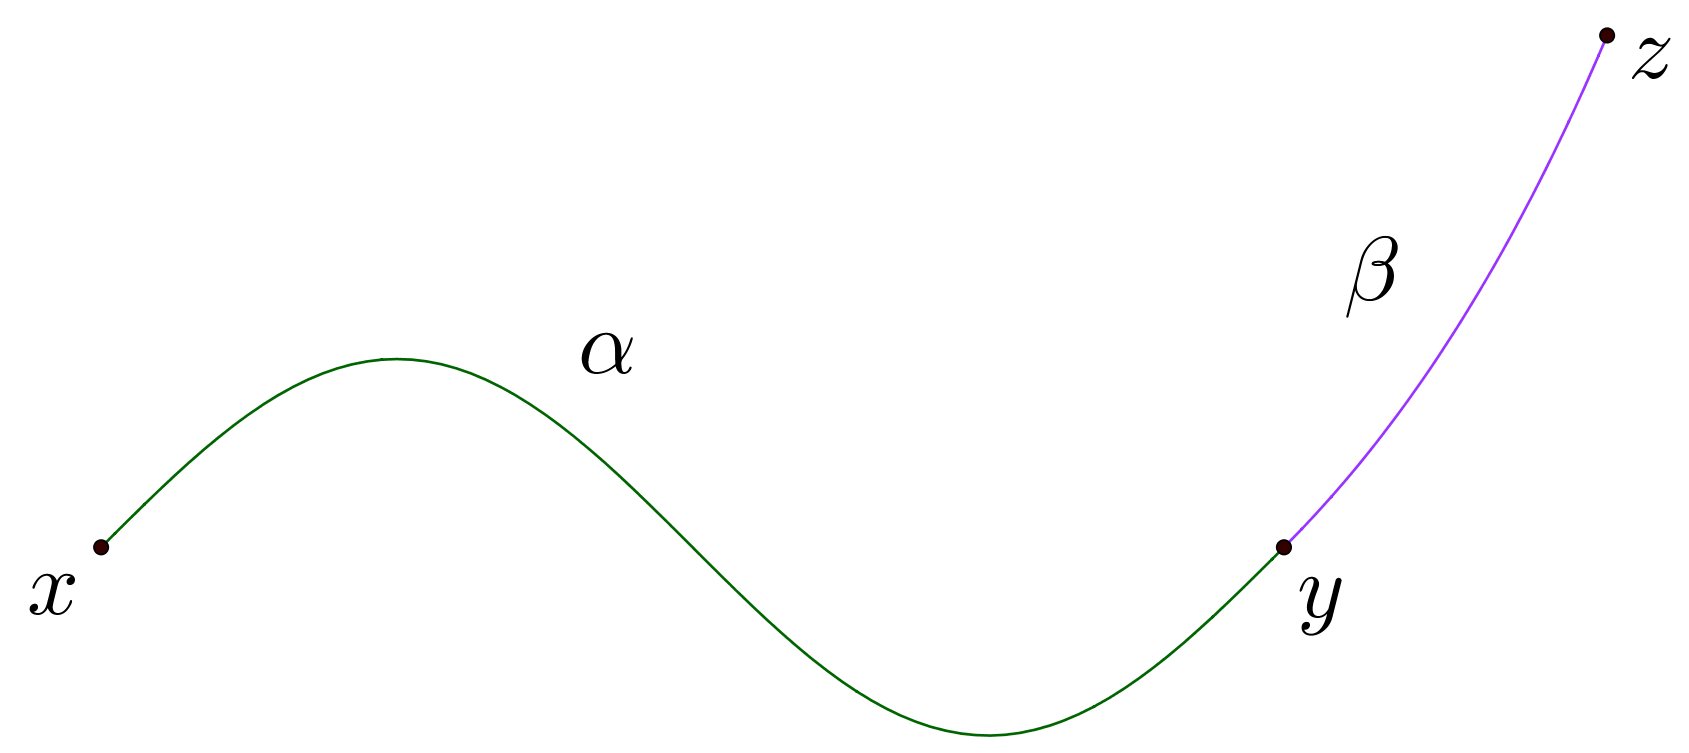
\includegraphics[scale=0.]{yux}
\end{figure}

\begin{nota} La yuxtaposición está bien definida en $t=\frac{1}{2}$ porque $\alpha(1)=\beta(0)=y$.
\end{nota}
\end{comment}

\begin{defi} Dos caminos se dicen \textbf{equivalentes} si existe una homotopía relativa al $\{0,1\}$ $H\func{I\times I}{X}$, esto es,  $H(t,0)=\alpha(t),H(t,1)=\beta(t)$ y por ser relativa $H(0,s)=x_0, H(1,s)=x_1$.
\end{defi}
\begin{comment}
\begin{figure}[h!]
	\centering
	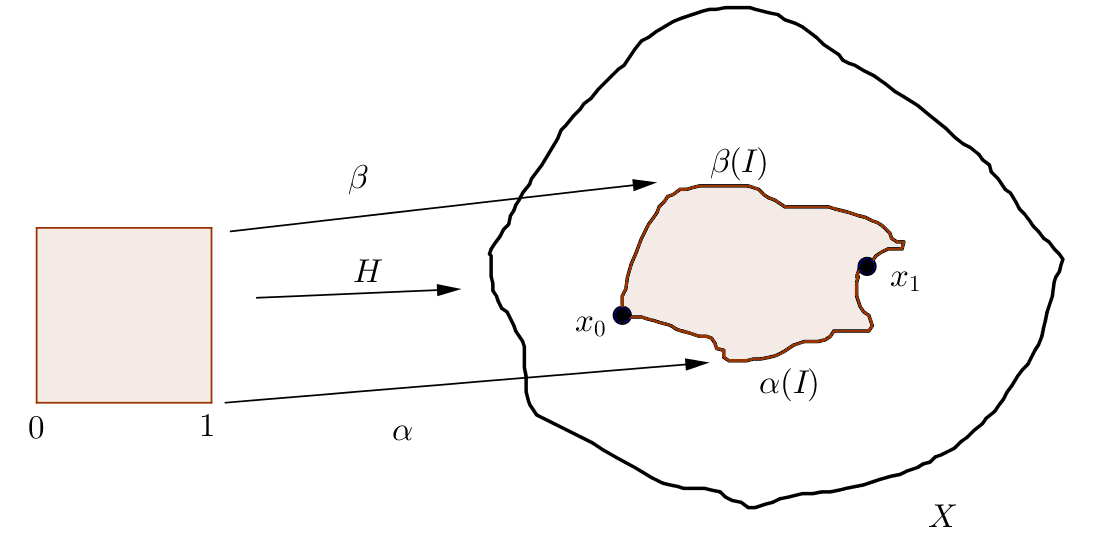
\includegraphics[scale=0.3]{caminoequivalente}
\end{figure}
\end{comment}
\begin{nota} Si $\alpha$ y $\beta$ son equivalentes escribimos $\alpha\sim\beta$ en lugar de $\alpha\simeq\beta$ relativamente a $\{0,1\}$.
\end{nota}

\begin{lemma} La yuxtaposición es compatible con la equivalencia de caminos.
\end{lemma}
\begin{comment}
\begin{dem}
Sean $\alpha\sim\alpha'$ y $\beta\sim\beta'$ con $\alpha(0)=\alpha'(0)=x$, $\alpha(1)=\alpha'(1)=\beta(0)=\beta'(0)=y$ y $\beta(1)=\beta'(1)=z$.\\
$\alpha\sim\alpha'\Rightarrow\exists\ H$ homotopía entre $\alpha$ y $\alpha'$ relativa a $\{0,1\}$.\\
$\beta\sim\beta'\Rightarrow\exists\ G$ homotopía entre $\beta$ y $\beta'$ relativa a $\{0,1\}$.

Sea $F\func{I\times I}{X}$ la homotopía resultante de ``unir'' las dos anteriores
\[
F(t,s)=\left\{\begin{array}{l c c}
H(2t,s) & si & 0\leq t\leq\frac{1}{2}\\
G(2t-1,s) & si &\frac{1}{2}\leq t\leq 1

\end{array}\right.
\]

\begin{figure}[h!]
	\centering
	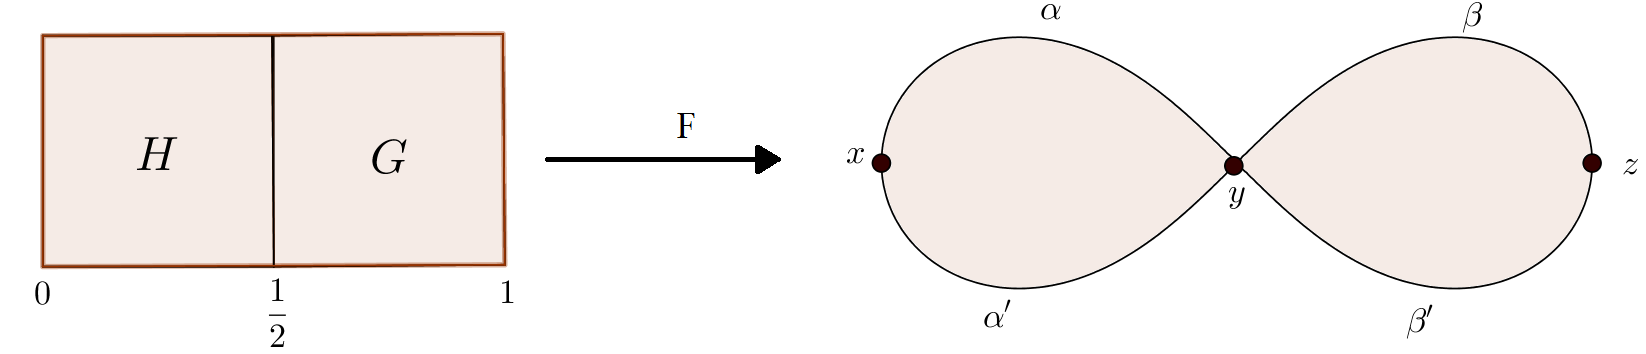
\includegraphics[scale=0.28]{yuxta}
\end{figure}

$F(\frac{1}{2},s)$ está bien definida pues, al ser $H$ y $G$ relativas al $\{0,1\}$ se tiene que $H(1,s)=y=G(0,s)$. Finalmente,
\[
F(t,0)=\left\{\begin{array}{lcc}
H(2t,0)=\alpha(2t) & si & 0\leq t\leq\frac{1}{2}\\
G(2t-1,0)=\beta(2t-1) & si & \frac{1}{2}\leq t\leq 1
\end{array}\right.
\]
que es justamente la yuxtaposición de $\alpha$ y $\beta$. Análogamente $F(t,1)=(\alpha'*\beta')(t)$. Finalmente,
\[
\left.\begin{array}{c}
F(0,s)=H(0,s)=x\\
F(1,s)=G(1,s)=z
\end{array}\right\}\Rightarrow \alpha*\beta\sim\alpha'*\beta'
\]
$\QED$
\end{dem}

\end{comment}

\begin{prop} Se cumplen las siguientes propiedades de la yuxtaposición con respecto a la equivalencia de caminos.
\begin{enumerate}
\item Propiedad asociativa: $(\alpha*\beta)*\gamma\sim\alpha*(\beta*\gamma)$

\item Elemento neutro: si $c_x$ es el camino constante $x$ y $\alpha$ es un camino entre $x$ e $y$, entonces $c_x*\alpha\sim\alpha\sim\alpha*c_y$.

\item Elemento inverso: si $\alpha$ es un camino entre $x$ e $y$ y $\overline{\alpha}\func{I}{X}$ es el camino $\overline{\alpha}(t)=\alpha(1-t)$ (camino opuesto), entonces $\alpha*\overline{\alpha}\sim c_x$ y $\overline{\alpha}*\alpha\sim c_y$.
\end{enumerate}
\end{prop}

%\vspace{1cm}
\begin{comment}
\begin{dem}Por definición tenemos
\begin{enumerate}
\item $\alpha*(\beta*\gamma)(t)=\left\{\begin{array}{lc}
\alpha(2t) & 0\leq t\leq\frac{1}{2}\\
\beta*\gamma(2t-1) & \frac{1}{2}\leq t\leq 1
\end{array}\right.=\left\{\begin{array}{lc}
\alpha(2t) & 0\leq t\leq\frac{1}{2}\\
\beta(4t-2) & \frac{1}{2}\leq t\leq\frac{3}{4}\\
\gamma(4t-3) & \frac{3}{4}\leq t\leq 1
\end{array}\right.$\\

$(\alpha*\beta)*\gamma(t)=\left\{\begin{array}{lc}
(\alpha*\beta)(2t) & 0\leq t\leq\frac{1}{2}\\
\gamma(2t-1) & \frac{1}{2}\leq t\leq 1
\end{array}\right.=\left\{\begin{array}{lc}
\alpha(4t) & 0\leq t\leq\frac{1}{4}\\
\beta(4t-1) & \frac{1}{4}\leq t\leq\frac{1}{2}\\
\gamma(2t-1) & \frac{1}{2}\leq t\leq 1
\end{array}\right.$\\
%\begin{figure}[h!]
%	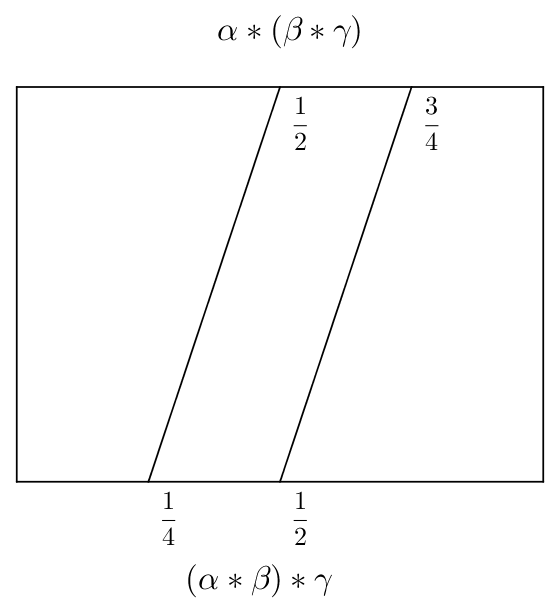
\includegraphics[scale=0.28]{dempropi2}
%\end{figure}
%\definecolor{zzttqq}{rgb}{0.6,0.2,0.} \fill[color=zzttqq,fill=zzttqq,fill opacity=0.1]

Sea por lo tanto
\[
F(t,s)=\left\{\begin{array}{lcc}
\alpha\left(\frac{4t}{s+1}\right) & si & 0\leq t\leq\frac{s+1}{4}\\
\beta\left(4t-(s+1)\right) & si & \frac{s+1}{4}\leq t\leq\frac{s+2}{4}\\
\gamma\left(\frac{4t-s-2}{2-s}\right) & si & \frac{s+2}{4}\leq t\leq 1
\end{array}\right.
\]
Se tiene que $F$ es una homotopía relativa a $\{0,1\}$ entre $F(t,0)=(\alpha*\beta)*\gamma(t)$ y $F(t,1)=\alpha*(\beta*\gamma)(t)$.

\item Para probar $c_x*\alpha\sim\alpha$ definimos la homotopía
\[
F(t,s)=\left\{\begin{array}{lcc}
x & si & 0\leq t\leq\frac{1-s}{2}\\
\alpha\left(\frac{2t+s-1}{s+1}\right) & si & \frac{1-s}{2}\leq t\leq 1
\end{array}\right.
\]
\definecolor{zzttqq}{rgb}{0.6,0.2,0.}
\begin{tikzpicture}[line cap=round,line join=round,>=triangle 45,x=1.0cm,y=1.0cm]
\clip(-4,-0.5) rectangle (8.29,2.5);
\draw (0.,0.)-- (4.,0.);
\draw (4.,0.)-- (4.,2.);
\draw (4.,2.)-- (0.,2.);
\draw (0.,2.)-- (0.,0.);
\draw (0.,2.)-- (2.,0.);
\draw (1.65,2.56) node[anchor=north west] {$\alpha$};
\draw (0.73,0.06) node[anchor=north west] {$c_x$};
\draw (2.86,0.06) node[anchor=north west] {$\alpha$};
\draw (1.9,0.09) node[anchor=north west] {$\frac{1}{2}$};
\fill[color=zzttqq,fill=zzttqq,fill opacity=0.1] (0,0)--(0,2)--(4,2)--(4,0)--cycle;
\end{tikzpicture}

La relación $\alpha\sim\alpha*c_y$ se demuestra de manera análoga.

\item Se tiene $\alpha*\overline{\alpha}(t)=\left\{\begin{array}{lc}
\alpha(2t) & 0\leq t\leq\frac{1}{2}\\
\overline{\alpha}(2t-1)=\alpha(2-2t) & \frac{1}{2}\leq t\leq 1
\end{array}\right.$\\

\definecolor{zzttqq}{rgb}{0.6,0.2,0.}
\begin{tikzpicture}[line cap=round,line join=round,>=triangle 45,x=1.0cm,y=1.0cm]
\clip(-4,-0.5) rectangle (8.29,2.5);
\draw (0.,0.)-- (4.,0.);
\draw (4.,0.)-- (4.,2.);
\draw (4.,2.)-- (0.,2.);
\draw (0.,2.)-- (0.,0.);
\draw (0.,2.)-- (2.,0.);
\draw (1.83,2.52) node[anchor=north west] {$c_x$};
\draw (2.88,0) node[anchor=north west] {$\overline{\alpha}$};
\draw (0.8,0) node[anchor=north west] {$\alpha$};
\draw (1.9,0.09) node[anchor=north west] {$\frac{1}{2}$};
\draw (2.,0.)-- (4.,2.);
\fill[color=zzttqq,fill=zzttqq,fill opacity=0.1] (0,0)--(0,2)--(4,2)--(4,0)--cycle;
\end{tikzpicture}

Entonces la ecuación
\[
F(t,s)=\left\{\begin{array}{lcc}
\alpha(2t(1-s)) & si & 0\leq t\leq\frac{1}{2}\\
\alpha((2-2t)(1-s)) & si & \frac{1}{2}\leq t\leq 1
\end{array}\right.
\]


define una homotopía relativa a $\{0,1\}$ entre $\alpha*\overline{\alpha}$ y $c_x$. Análogamente se encuentra una homotopía relativa a $\{0,1\}$ entre $\overline{\alpha}*\alpha$ y $c_y$.
\end{enumerate}
\end{dem}
\end{comment}
\section{Grupo Fundamental}
Sea $\Omega(X,x_0)$ el conjunto de lazos en $x_0$ de $X$, esto es $\{\alpha\func{I}{X};\ \alpha(0)=\alpha(1)=x_0\}$. Definimos a continuación el conjunto cociente $\pi_1(X,x_0)=\Omega(X,x_0)/\sim$ por la relación de equivalencia de caminos. Definimos además el producto de clases $[\alpha][\alpha']=[\alpha*\alpha']$, el cual está bien definido pues hemos visto que $\alpha\sim\beta$ y $\alpha'\sim\beta'\Rightarrow\alpha*\alpha'\sim\beta*\beta'$.

\begin{prop} $\pi_1(X,x_0)$ es un grupo.
\end{prop}
\begin{comment}
\begin{dem}\
\begin{enumerate}
\item Asociatividad:
\[
[\alpha]([\beta][\gamma])=[\alpha*(\beta*\gamma)]=[(\alpha*\beta)*\gamma]=([\alpha][\beta])[\gamma]
\]
\item Elemento neutro: $[c_{x_0}]$
\[
[\alpha][c_{x_0}]=[\alpha* c_{x_0}]=[\alpha]=[c_{x_0}*\alpha]=[c_{x_0}][\alpha]
\]
\item Elemento inverso: $[\overline{\alpha}]$
\[
[\alpha][\overline{\alpha}]=[\alpha*\overline{\alpha}]=[c_{x_0}]=[\overline{\alpha}*\alpha]=[\overline{\alpha}][\alpha]
\]
\end{enumerate}
\end{dem}
\end{comment}
\begin{defi}
A $\pi_1(X,x_0)$ se le llama grupo fundamental del espacio $X$ en $x_0$.
\end{defi}

\begin{prop} Sea $f\func{X}{Y}$ una aplicación continua. Entonces $f$ induce un homomorfismo de grupos:
\begin{gather*}
f_*\func{\pi_1(X,x_0)}{\pi_1(Y,f(x_0))}\\
f_*[\alpha]=[f\circ\alpha]
\end{gather*}

\end{prop}


\begin{comment}
\begin{dem}\
\begin{itemize}
\item $f_*$ está bien definida, pues la relación de homotopía relativa a $\{0,1\}$ es compatible con la composición:
\[
f\circ\alpha\simeq f\circ\alpha'\textit{ relativamente a }\{0,1\}\Rightarrow f\alpha\sim f\alpha'\Leftrightarrow[f\alpha]=[f\alpha']
\]
\item $f_*$ es homomorfismo, pues la yuxtaposición de caminos es compatible con la composición:
\[
f_*([\alpha][\alpha'])=f_*([\alpha*\alpha'])=[f\circ(\alpha*\alpha')]=[f\alpha*f\alpha']=[f\alpha][f\alpha']=f_*[\alpha] f_*[\alpha']
\]
$\QED$
\end{itemize}
\end{dem}
\end{comment}
\begin{prop} Se cumplen
\begin{enumerate}
\item Si $X\overset{f}{\longrightarrow}Y\overset{g}{\longrightarrow}Z$ entonces $(g\circ f)_*=g_*f_*$.
\item $Id_*=Id$
\end{enumerate}
\end{prop}
\begin{comment}
\begin{dem}
\begin{enumerate}
\item $(g\circ f)_*[\alpha]=[gf\alpha]=g_*[f\alpha]=g_*f_*[\alpha]$
\item $Id_*[\alpha]=[Id\alpha]=[\alpha]$
$\QED$
\end{enumerate}
\end{dem}
\end{comment}
\begin{consec} Si $f\func{X}{Y}$ es homeomorfismo entonces $f_*$ es isomorfismo.
\end{consec}
\begin{comment}
\begin{dem}
Sea $f^{-1}\func{Y}{X}$. Se tiene el siguiente diagrama.
\[
\pi_1(X,x_0)\overset{f_*}{\longrightarrow}\pi_1(Y,f(x_0))\overset{(f^{-1})_*}{\longrightarrow}\pi_1(X,x_0)
\]
Se cumple
\begin{gather*}
f_*\circ(f^{-1})_*=(f\circ f^{-1})_*=Id_*=Id\\
(f^{-1})_*\circ f_*=(f^{-1}\circ f)_*=Id_*=Id
\end{gather*}
Por lo tanto $f_*$ es isomorfismo y su inversa es $(f^{-1})_*$. $\QED$
\end{dem}
\end{comment}


\vspace{0.4cm}

\begin{nota} Si $f\func{X}{Y}$ es una equivalencia de homotopía, entonces $\exists\ g\func{Y}{X}$ continua tal que $f\circ g\simeq Id_X$ y $g\circ f\simeq Id_Y$
\[
x_0\overset{f}{\longmapsto}f(x_0)\overset{g}{\longmapsto}g(f(x_0))
\]
Nótese que $g(f(x_0))$ no tiene por qué ser $x_0$. Tenemos entonces
\[
\pi_1(X,x_0)\overset{f_*}{\longrightarrow}\pi_1(Y,f(x_0))\overset{g*}{\longrightarrow}\pi_1(X,g(f(x_0)))
\]




Si $H$ es una homotopía entre $Id_X$ y $g\circ f$, tenemos que $\gamma(t)=H(x_0,t)$ es un camino entre $x_0$ y $g(f(x_0))$. 
\end{nota}

\vspace{0.4cm}

\begin{prop}
Sea $\gamma\func{I}{X}$ un camino entre $x_0$ y $x_1$. Entonces existe un isomorfismo
\[
\gamma_\sharp\func{\pi_1(X,x_1)}{\pi_1(X,x_0)}
\]
dado por
\[
\gamma_\sharp([\alpha])=[(\gamma*\alpha)*\overline{\gamma}]=[\gamma*(\alpha*\overline{\gamma})].
\]
Además, si $\gamma$ es equivalente a $\gamma'$, $\gamma_\sharp=\gamma'_\sharp$.
\end{prop}
\begin{comment}
\begin{dem}\


\begin{tikzpicture}[line cap=round,line join=round,>=triangle 45,x=1.0cm,y=1.0cm]
\clip(-3,2) rectangle (2,5);
\draw [line width=1.6pt] (-2.36,2.66)--  (-2.36,2.66)-- (-2.34,2.72)-- (-2.28,2.76)-- (-2.22,2.78)-- (-2.16,2.84)-- (-2.1,2.88)-- (-2.04,2.9)-- (-1.98,2.92)-- (-1.92,2.94)-- (-1.84,2.94)-- (-1.78,2.96)-- (-1.7,2.96)-- (-1.64,2.98)-- (-1.56,2.98)-- (-1.5,3.)-- (-1.44,3.02)-- (-1.38,3.04)-- (-1.3,3.04)-- (-1.24,3.06)-- (-1.16,3.08)-- (-1.1,3.1)-- (-1.04,3.12)-- (-0.98,3.14)-- (-0.9,3.16)-- (-0.82,3.18)-- (-0.76,3.2)-- (-0.7,3.22)-- (-0.64,3.26)-- (-0.56,3.26)-- (-0.5,3.28)-- (-0.44,3.32)-- (-0.38,3.34)-- (-0.32,3.38)-- (-0.24,3.4)-- (-0.18,3.44)-- (-0.12,3.5)-- (-0.06,3.52)--  (-0.02,3.56)--  (-0.02,3.56)-- (-0.02,3.64)-- (-0.02,3.72)-- (-0.02,3.8)-- (-0.02,3.88)-- (-0.02,3.98)-- (0.,4.08)-- (0.,4.16)-- (0.04,4.22)-- (0.06,4.3)-- (0.08,4.36)-- (0.14,4.42)-- (0.2,4.48)-- (0.26,4.5)-- (0.32,4.54)-- (0.38,4.56)-- (0.46,4.56)-- (0.54,4.56)-- (0.62,4.56)-- (0.7,4.56)-- (0.78,4.56)-- (0.84,4.54)-- (0.9,4.52)-- (0.96,4.48)-- (1.02,4.44)-- (1.08,4.38)-- (1.1,4.32)-- (1.12,4.24)-- (1.14,4.18)-- (1.14,4.1)-- (1.16,4.02)-- (1.16,3.94)-- (1.14,3.86)-- (1.08,3.8)-- (1.02,3.76)-- (0.96,3.72)-- (0.9,3.68)-- (0.84,3.64)-- (0.78,3.62)-- (0.72,3.6)-- (0.64,3.6)-- (0.56,3.6)-- (0.48,3.6)-- (0.4,3.6)-- (0.34,3.62)-- (0.28,3.64)-- (0.2,3.64)-- (0.12,3.64)-- (0.06,3.6)-- (0.,3.56);
\draw (-2.64,2.5) node[anchor=north west] {$x_0$};
\draw (0.,3.66) node[anchor=north west] {$x_1$};
\draw (1.26,4.4) node[anchor=north west] {$\alpha$};
\draw (-1.46,3.6) node[anchor=north west] {$\gamma$};
\draw [line width=1.6pt] (0.58,3.62)-- (0.58,3.62)-- (0.6,3.68)-- (0.64,3.74)--  (0.6,3.62)--  (0.6,3.62)-- (0.64,3.56)-- (0.7,3.52);
\begin{scriptsize}
\draw [fill=black] (-2.354,2.678) circle (2.5pt);
\draw [fill=black] (-0.02,3.58) circle (2.5pt);
\end{scriptsize}
\end{tikzpicture}

La aplicación $\gamma_\sharp$ está bien definida: $\alpha\sim\alpha'\Rightarrow\gamma*\alpha*\overline{\gamma}\sim\gamma*\alpha'*\overline{\gamma}$. Vamos a comprobar que es homomorfismo:
\begin{gather*}
\gamma_\sharp([\alpha][\alpha'])=\\
=\gamma_\sharp([\alpha*\alpha'])=[\gamma*(\alpha*\alpha')*\overline{\gamma}]=[\gamma*\alpha*\underbrace{\overline{\gamma}*\gamma}_{\sim c_{x_0}}*\alpha'*\overline{\gamma}]=\\
\overset{(1)}{=}[(\gamma*\alpha*\overline{\gamma})*(\gamma*\alpha'*\overline{\gamma})]
=\gamma_\sharp[\alpha]\gamma_\sharp[\alpha'].
\end{gather*}
En $(1)$ se usa la asociatividad de la yuxtaposición.
Para probar que es isomorfismo veamos que $\gamma^{-1}_\sharp=\overline{\gamma}_\sharp$:
\begin{gather*}
\gamma_\sharp\cdot\overline{\gamma}_\sharp([\alpha])=\gamma_\sharp([\overline{\gamma}*\alpha*\underset{\underset{\gamma}{\verteq}}{\overline{\overline{\gamma}}}])=[\underbrace{\gamma*\overline{\gamma}}_{\sim c_{x_0}}*\alpha*\underbrace{\gamma*\overline{\gamma}}_{\sim c_{x_0}}]=[c_{x_0}*\alpha*c_{x_0}]=[\alpha].
\end{gather*}
Análogamente se prueba que $\overline{\gamma}_\sharp\gamma_\sharp([\alpha])=[\alpha]$.$\QED$
\end{dem}
\end{comment}
\begin{coro}
Todo lazo $\gamma$ en $x_0$ induce un automorfismo de $\pi_1(X,x_0)$ dado por conjugación, es decir, a cada elemento $[\alpha]$ se le hace corresponder $[\gamma][\alpha][\gamma]^{-1}$.
\end{coro}

\begin{prop}
Sea $H$ una homotopía $H\func{X\times I}{Y}$ entre $f,g\func{X}{Y}$. Dado $x_0\in X$, sea $\gamma\func{I}{X}$ el camino $\gamma(t)=H(x_0,t)$. Este camino va de $f(x_0)=H(x_0,0)$ a $g(x_0)=H(x_0,1)$. Tenemos el diagrama conmutativo
\[
\begin{tikzcd}
\pi_1(X,x_0)\arrow[d,"g_*"] \arrow[r, "f_*"] &  \pi_1(Y,f(x_0))\arrow[dl,"\cong"',"\overline{\gamma}_\sharp"] \\
\pi_1(Y,g(x_0))\arrow[ur, dashrightarrow,"\gamma_\sharp"', bend right=30]  %, bend right=30
\end{tikzcd}
\]
\end{prop}
\begin{comment}
\begin{dem}[con la inversa, $\overline{\gamma}_\sharp$]
Sea $[\alpha]\in\pi_1(X,x_0)$. Sea $G=H\circ(\alpha\times Id)$
\begin{center}


\begin{tikzpicture}[line cap=round,line join=round,>=triangle 45,x=1.0cm,y=1.0cm]
\clip(-4.3,-1) rectangle (10,1);
\draw (0.,0.)-- (0.,1.);
\draw (0.,1.)-- (-1.,1.);
\draw (-1.,1.)-- (-1.,0.);
\draw (-1.,0.)-- (0.,0.);
\draw [->] (0.32,0.5) -- (2,0.5);
\draw [->] (4.,0.5) -- (6,0.5);
\draw (-1.1,0.) node[anchor=north west] {$I\times I$};
\draw (0.4,1) node[anchor=north west] {$\alpha\times Id$};
\draw (2.2,0.8) node[anchor=north west] {\Huge{\Large{$X\times I$}}};
\draw (4.6,1.) node[anchor=north west] {$H$};
\draw (6.2,0.8) node[anchor=north west] {\Huge{\Large{$Y$}}};
\end{tikzpicture}
\end{center}

Se define $F\func{I\times I}{Y}$ de la siguiente forma
\[
F(t,s)=\left\{\begin{array}{lcc}
\overline{\gamma}(2t) & si & 0\leq t\leq\frac{1-s}{2}\\
G\left(\frac{4t+2s-2}{2s+1},s\right) & si & \frac{1-s}{2}\leq t\leq\frac{s+3}{4}\\
\gamma(4t-3) & si & \frac{s+3}{4}\leq t\leq 1
\end{array}\right.
\]
$F$ hace que $\overline{\gamma}*((f\circ\alpha)*\gamma)\sim g\circ\alpha\underset{def}{\Longrightarrow}\overline{\gamma}_\sharp f_*[\alpha]=g_*[\alpha]$.
\begin{center}
\definecolor{zzttqq}{rgb}{0.6,0.2,0.}
\begin{tikzpicture}[line cap=round,line join=round,>=triangle 45,x=1.0cm,y=1.0cm]
\clip(0,-1) rectangle (3.2,2.5);
\draw (0.,0.)-- (3.,0.);
\draw (3.,0.)-- (3.,2.);
\draw (3.,2.)-- (0.,2.);
\draw (0.,2.)-- (0.,0.);
\draw (0.,2.)-- (1.0466666666666666,0.);
\draw (2.006666666666666,0.)-- (3.,2.);
\draw (0.54,0.)-- (0.3933333333333338,-0.14666666666666414);
\draw (0.54,0.)-- (0.42,0.16);
\draw (2.54,0.)-- (2.3933333333333338,-0.14666666666666414);
\draw (2.54,0.)-- (2.42,0.16);
\draw (0.5488269413601512,0.9512860993118131)-- (0.31333333333333385,1.04);
\draw (0.5488269413601512,0.9512860993118131)-- (0.5933333333333337,1.2266666666666668);
\draw (2.5291978384031037,1.0520761847042361)-- (2.2733333333333325,0.96);
\draw (2.5291978384031037,1.0520761847042361)-- (2.5933333333333324,0.8);
\draw (1.2466666666666666,2.4) node[anchor=north west] {$g\circ\alpha$};
\draw (0.1,0.6133333333333345) node[anchor=north west] {$\overline{\gamma}$};
\draw (0.7266666666666669,1.4) node[anchor=north west] {$\overline{\gamma}$};
\draw (2.446666666666666,0.5733333333333346) node[anchor=north west] {$\gamma$};
\draw (2.2733333333333325,1.68) node[anchor=north west] {$\gamma$};
\draw (1.38,1.24) node[anchor=north west] {$G$};
\draw (1.1666666666666665,0.) node[anchor=north west] {$f\circ\alpha$};
\fill[color=zzttqq,fill=zzttqq,fill opacity=0.1] (0,0)--(0,2)--(3,2)--(3,0)--cycle;
\end{tikzpicture}

\end{center}
\end{dem}
\end{comment}
\begin{coro}\label{coro1AQ}
Si $f\simeq Id$, entonces $f_*=\gamma_\sharp$.
\end{coro}
\begin{coro}
Si $f\func{X}{Y}$ es una equivalencia de homotopía, entonces $f_*\func{\pi_1(X,x_0)}{\pi_1(Y,f(x_0))}$ es isomorfismo.
\end{coro}
\begin{comment}
\begin{dem}
Como $f$ es equivalencia de homotopía $\exists g\func{Y}{X}$ tal que
\begin{itemize}

\item $f\circ g\overset{G}{\simeq}Id_Y$
\item $g\circ f\overset{F}{\simeq}Id_X$
\end{itemize}
Tenemos para el camino $\gamma(t)=F(x_0,t)$ que $g_*\circ f_*=(g\circ f)_*=\gamma_\sharp$ por el Corolario \ref{coro1AQ}.
\[
\begin{tikzcd}
\pi_1(X,x_0)\arrow[r, "f_*"]\arrow[rr, "(g\circ f)_*=\gamma_\sharp", bend right=20] &  \pi_1(Y,f(x_0))\arrow[r,"g_*"] & \pi_1(X,g(f(x_0)))
\end{tikzcd}
\]

Entonces $g_*\circ f_*$ isomorfismo $\Rightarrow f_*$ inyectiva y $g_*$ sobreyectiva. Análogamente, para el camino $\eta(t)=G(f(x_0),t)$ tenemos que $g_*\circ f_*=(g\circ f)_*=\eta_\sharp$.
\[
\begin{tikzcd}
\pi_1(Y,f(x_0))\arrow[r, "g_*"]\arrow[rr, "(f\circ g)_*=\eta_\sharp", bend right=20] & \pi_1(X,g(f(x_0))) \arrow[r,"f_*"] & \pi_1(Y,f(g(f(x_0))))
\end{tikzcd}
\]
por lo que $g_*$ inyectiva y $f_*$ sobreyectiva. En consecuencia, tanto $g_*$ como $f_*$ son biyectivas, ergo isomorfismos. $\QED$

\end{dem}
\end{comment}
\begin{coro}
Si $A\subseteq X$ es un retracto de deformación de $X$, entonces la inclusión $i:A\hookrightarrow X$ induce un isomorfismo $i_*\func{\pi_1(A,x_0)}{\pi_1(X,x_0)}$. En particular, los lazos que representan generadores de $\pi_1(A,x_0)$ también representan generadores de $\pi_1(X,x_0)$.
\end{coro}
\begin{comment}
\begin{dem}
Sea $i:A\hookrightarrow X$ la inclusión y $r\func{X}{A}$ la correspondiente retracción. Si probamos que las composiciones indicadas en los siguientes diagramas
\[
\begin{tikzcd}
\pi_1(A,x_0)\arrow[r, "i_*"] & \pi_1(X,x_0)\arrow[r, "r_*"] & \pi_1(A,x_0)\\
\pi_1(X,x_0)\arrow[r, "r_*"] & \pi_1(A,x_0)\arrow[r, "i_*"] & \pi_1(X,x_0)
\end{tikzcd}
\]
son la identidad, deduciremos que $r_*$ tiene a $i_*$ como inversa y que por lo tanto es isomorfismo. En primer lugar, usando la definición de retracto
\[
r_*\circ i_*=(r\circ i)_*=Id_*=Id.
\]
En segundo lugar, usamos que $i\circ r\simeq Id$
\[
i_*\circ r_*=(i\circ r)_*=[i\circ r]=[Id]=Id_*=Id.
\]$\QED$
\end{dem}
\end{comment}
Si $X$ es contráctil entonces tiene el mismo tipo de homotopía que un espacio unipuntual  $\{p\}$ y por tanto, 
\begin{coro}
Si $X$ es contractil entonces $\pi_1(X,p) \cong \pi_1(\{p\},p) = \{1\}$.  
\end{coro}

\begin{defi} Si $X$ es un espacio conexo por caminos y $\pi_1(X,x_0)=\{1\}$, entonces se dice que $X$ es \textbf{simplemente conexo} o \textbf{1-conexo}.
\end{defi}
\begin{comment}
\begin{ejer}
Si $r:X\to A$ es una retracción e $i:A\hookrightarrow X$ es la inclusión, entonces $i_*$ es inyectiva y $r_*$ es sobreyectiva.
\end{ejer}
\begin{solucion}
Por ser $r$ una retracción se tiene que $r\circ i =Id_A$, por lo que $r_*\circ i_*=(r\circ i)_*=Id_{\pi_(A)}$. De este hecho se deducen los dos resultados. Por un lado $r_*$ es sobreyectiva por tener inversa a la derecha y por otro lado $i_*$ es inyectiva por tener inversa a la izquierda. \qed
\end{solucion}
\end{ejer}
\begin{prop} Sean $X$ e $Y$ espacios topológicos, entonces
\[
\pi_1(X\times Y, (x_0,y_0))\cong\pi_1(X,x_0)\times\pi_1(Y,y_0).
\]
\end{prop}
\begin{comment}
\begin{dem}
Sea $\alpha\func{I}{X\times Y}$ un lazo y las correspondientes proyecciones $p_1$ y $p_2$
\[
\begin{tikzcd}
X\times Y \ar[r, "p_1"]\ar[d, "p_2"] & X\\
Y
\end{tikzcd}
\]
dadas por $p_1(x,y)=x$ y $p_2(x,y)=y$. Ambas son continuas para la topología producto (probar como ejercicio). Consideremos los siguientes homomorfismos:
\begin{gather*}
p_{1*}\func{\pi_1(X\times Y, (x_0,y_0))}{\pi_1(X,x_0)},\\
p_{2*}\func{\pi_1(X\times Y, (x_0,y_0))}{\pi_1(Y,y_0)}.
\end{gather*}

\begin{figure}[h!]
	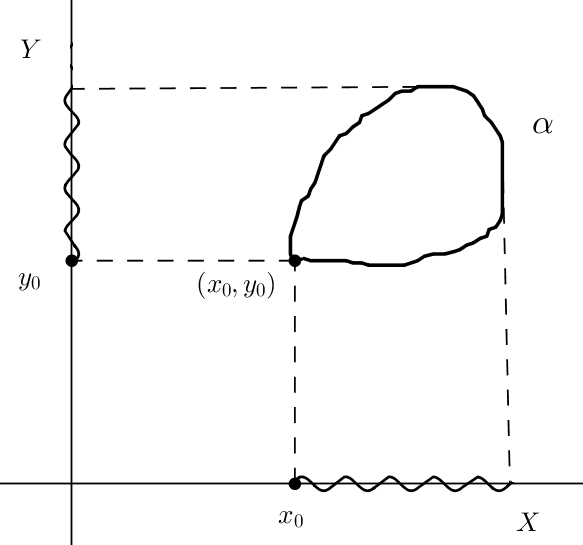
\includegraphics[scale=0.35]{proy}
\end{figure}

Sea
\begin{gather*}
\psi\func{\pi_1(X\times Y, (x_0,y_0))}{\pi_1(X,x_0)\times\pi_1(Y,y_0)},\\
\qquad[\alpha]\longmapsto(p_{1*}[\alpha],p_{2*}[\alpha])=([p_1\circ\alpha],[p_2\circ\alpha]).
\end{gather*}
Es fácil comprobar que $\psi$ es homomorfismo para el producto $(a,b)\cdot(a',b')=(aa',bb')$. Veamos que es isomorfismo:
\begin{itemize}
\item $\psi$ sobreyectiva.\\
Sean $[\varepsilon]\in\pi_1(X,x_0),[\eta]\in\pi_1(Y,f(x_0))$. Definimos $\varepsilon\times\eta\func{I}{X\times Y}$ como $(\varepsilon\times\eta)(t)=(\varepsilon(t),\eta(t))$ que es continua para la topología producto (comprobar como ejercicio). Se cumple
\[
(\varepsilon\times\eta)(0)=(\varepsilon(0),\eta(0))=(x_0,y_0)=(\varepsilon\times\eta)(1),
\]
por lo que $\varepsilon\times\eta$ es un lazo en $X\times Y$ de punto base $(x_0,y_0)$ para el cual
\[
\psi([\varepsilon,\eta])=([p_1\circ(\varepsilon,\eta)],[p_2\circ(\varepsilon,\eta)])=([\varepsilon],[\eta]).
\]
\item $\psi$ inyectiva.\\
Supongamos que $\psi([\alpha])=\psi([\beta])$. Esto implica lo siguiente:
\begin{gather*}
[p_1\circ\alpha]=[p_1\circ\beta]\Rightarrow p_1\alpha\sim p_1\beta,\\
[p_2\circ\alpha]=[p_2\circ\beta]\Rightarrow p_2\alpha\sim p_2\beta.
\end{gather*}

Por tanto existen homotopías $F,G\func{I\times I}{X}$ tales que
\begin{gather*}
F(t,0)=p_1\alpha(t), F(t,1)=p_1\beta(t) \mbox{ y } F(0,s)=x_0=F(1,s),\\
G(t,0)=p_2\alpha(t), G(t,1)=p_2\beta(t) \mbox{ y } G(0,s)=y_0=G(1,s).
\end{gather*}


%\begin{gather*}
%F\func{I\times I}{X}\\
%\left.
%\begin{array}{c}
%F(t,0)=p_1\alpha(t)\\
%F(t,1)=p_1\beta(t)
%\end{array}\right\}F(0,s)=x_0=F(1,s)
%\end{gather*}

%\begin{gather*}
%G\func{I\times I}{Y}\\
%\left.
%\begin{array}{c}
%G(t,0)=p_2\alpha(t)\\
%G(t,1)=p_2\beta(t)
%\end{array}\right\}G(0,s)=y_0=G(1,s)
%\end{gather*}

Sea $H\func{I\times I}{X\times Y}$ definida como $H(t,s)=(F(t,s),G(t,s))$ (como ejercicio, probar que es continua para la topología producto). Se cumplen
\begin{gather*}
H(t,0)=(p_1\alpha(t),p_2\alpha(t))=\alpha(t),\\
H(t,1)=(p_1\beta(t),p_2\beta(t))=\beta(t),\\
H(0,s)=(x_0,y_0)=H(1,s).
\end{gather*}
Por todo ello, $\alpha\sim\beta$, es decir $[\alpha]=[\beta]$, como queríamos demostrar. $\QED$
\end{itemize}
\end{dem}
\end{comment}
\end{document} 